\documentclass{article}
\usepackage{graphicx}

\title{Special Numbers in Euler’s Identity}
\author{Joyce Huang}

\begin{document}

\maketitle
In math, not all numbers are of equal importance. Some have very special and unique properties that constantly show up in formulas and theorems. Five of these special numbers are $0$, $1$, $i$, $\pi$, and $e$.

\begin{center}
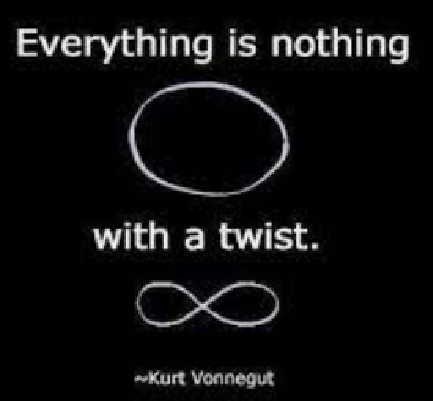
\includegraphics[scale=0.6]{images/specialnum0.png}
\end{center}

$0$ represents the quantity of nothing. Societies from all over the world invented the concept independently millennia ago, and it is extremely unlike any other number. 0 is neither positive nor negative, it cannot be a divisor, and so much more. It is also an additive identity, meaning   $x + 0 = x$ for all $x$. 


$1$ represents a single unit or quantity. The first natural number, it too is very special. $1$ is neither prime nor composite and it only has one divisor, which is itself. Also, $1$ is a multiplicative identity, meaning $x\times 1 = x$ for all $x$. 

For a long time, it was accepted as fact that the square of every number is nonnegative, and that one cannot take the square root of a negative number. However, the introduction of the number $i$ into mathematics brought about entirely new branches of math and countless new discoveries. $i$ is the square root of $-1$, and is called an imaginary number. Numbers of the form $a + bi$, where a and b are real numbers, are called complex numbers, and can be graphed on a coordinate plane. So, the discovery of $i$ quite literally introduced a whole new dimension of numbers.
\begin{center}
    
\includegraphics[scale=0.8]{images/specialnum2.png}
\end{center}
As mathematicians began to study circles, their curiosities were sparked by the relationship between different lengths in a circle, namely the ratio between the circumference and the diameter. It seemed that no matter the size of the circle, the ratio was always the same, so the question shifted to finding the exact value of that ratio. Of course, the exact value could never have been found, since $\pi$ is an irrational number. It is also a transcendental number, meaning it is not the root of any polynomial of finite degree with rational coefficients. $\pi$ has become one of the most well-known irrational numbers, with most people knowing at least several of its first digits and others striving to memorize as much of it as they can for fun.
\begin{center}
    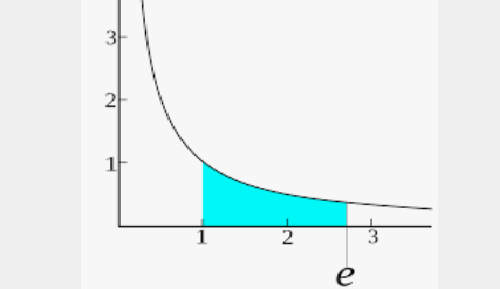
\includegraphics[scale=0.8]{images/specialnum3.png}
\end{center}
The constant $e$, also known as Euler’s number, has been widely used in number theory, algebra, statistics, and more since the early 17th century. Swiss mathematician Jacob Bernoulli discovered its value in 1683, but it had been referred to in a list of logarithms in base $e$, the natural logarithm, as early as 1618.

When Bernoulli discovered e, he had been trying to find the value of
\[\lim_{n\rightarrow\infty} \left(1+\frac{1}{n}\right)^n.\]
This expression might look familiar to you; Bernoulli discovered it while studying compound interest. As the frequency the interest is added to a starting value of $\$1$ increases infinitely, the money approaches $\$2.71828…$, which is the value of $e$. 

Another Swiss mathematician, Leonhard Euler, became engrossed in the number and discovered that it is the value of the sum.
\[e=\sum_{n=0}^{\infty}\frac{1}{n!}=1+\frac{1}{1}+\frac{1}{1\cdot 2} + ...\]
Euler also had many more discoveries related to $e$, including Euler’s formula, 
\[e^{ix}=\cos x + i\sin x,\]
a special case of which is \emph{Euler’s identity}.

\begin{center}
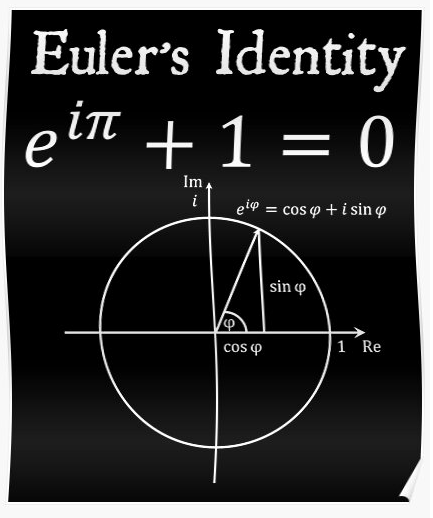
\includegraphics[scale=0.75]{images/specialnum1.png}
\end{center}

Euler’s identity is Euler’s formula when $x = \pi$. The equation then becomes
\[e^{i\pi}+1=0.\]

One might notice that there are 5 distinct numbers in this equation, and they happen to be the special numbers discussed in the article! Not only that, this identity includes each of the basic arithmetic functions addition, multiplication, and exponentiation exactly once. 

Euler’s identity is truly very special and combines five very special elements in it.
\end{document}